\documentclass{../TechDoc}

\title{Анализ поведения временных систем с помощью динамических метрических графов.}
\author{Студент группы БПИ172}{А. А. Измайлов}
\academicTeacher{Доцент департамента программной инженерии
	факультета компьютерных наук}{Л. В. Дворянский}

\documentTitle{Руководство оператора}
\documentCode{RU.17701729.04.01-01 34 01-1}

\begin{document}
	\maketitle
	\tableofcontents
	
	\section{Назначение программы}
	\subsection{Область применения}
	Программа для проверки поведенческих свойств сетей Петри с помощью редукций - программа, которая применяет редукции к обычной сети Петри, а также проводит анализ на живость и ограниченность.
	
	\subsection{Информация о функциях и принципе эксплуатации программы}
	Программа используется для приведения сети Петри к редуцированному виду, а также для анализа. Для работы программе нужен файл с сетью Петри в формате PNML. Результат работы программы можно использовать в других программах-анализаторах.
	
	\subsection{Уровень подготовки пользователя}
	Требуемая квалификация пользователя – оператор ПК, с пониманием сетей Петри.
	
	\section{Условия выполнения программы}
	\subsection{Требования к аппаратным средствам}
	\begin{itemize}
		\item Процессор архитектуры AMD или Intel с частотой не менее 2 266 МГц;
		\item Не менее 512 МБ ОЗУ;
		\item Не менее 200МБ на жестком диске;
		\item Клавиатура;
	\end{itemize}
	
	\subsection{Требования к информационной и программной совместимости}
	\begin{itemize}
		\item Одна из ниже перечисленных операционных систем:
		\begin{itemize}
			\item Windows 10
			\item Windows 8.x (настольная версия)
			\item Windows 7 с пакетом обновления 1 (SP1)
			\item Windows Vista SP2
			\item Windows Server 2008 R2 с пакетом обновления 1 (SP1) (64-разрядная версия)
			\item Windows Server 2012 и 2012 R2 (64-разрядная версия)
			\item Mac OS X 10.8.3+, 10.9+
			\item Oracle Linux 5.5+1
			\item Oracle Linux 6.x (32-разрядная версия), 6.x (64-разрядная версия)2
			\item Oracle Linux 7.x (64-разрядная версия)2
			\item Red Hat Enterprise Linux 5.5+1, 6.x (32-разрядная версия), 6.x (64-разрядная версия)2
			\item Red Hat Enterprise Linux 7.x (64-разрядная версия)2
			\item Suse Linux Enterprise Server 10 SP2+, 11.x
			\item Suse Linux Enterprise Server 12.x (64-разрядная версия)2
			\item Ubuntu Linux 12.04 LTS, 13.x, 14.x, 15.x, 16.x, 18.x
		\end{itemize}
		\item Установленная Java SE Runtime Environment 11 или выше
	\end{itemize}

	\subsection{Состав программы}
	\begin{itemize}
		\item bash-скрипт tapn-to-mg для запуска на Unix системах.
		\item bat-скрипт tapn-to-mg.bat для запуска на OS  Windows.
		\item jar архивы, необходимые для запуска программы
		\begin{itemize}
			\item AppleJavaExtensions.jar
			\item cli-app-0.0.jar
			\item commons-beanutils-1.9.2.jar
			\item commons-cli-1.2.jar
			\item commons-collections-3.2.2.jar
			\item commons-digester-1.8.1.jar
			\item commons-logging-1.2.jar
			\item commons-validator-1.5.1.jar
			\item converters-0.0.jar
			\item guava-19.0.jar
			\item jackson-core-2.10.3.jar
			\item jgrapht-core-1.4.0.jar
			\item jheaps-0.11.jar
			\item jna.jar
			\item json-20160810.jar
			\item log4j-api-2.13.1.jar
			\item log4j-core-2.13.1.jar
			\item metric-graphs-0.0.jar
			\item org.everit.json.schema-1.5.1.jar
			\item picocli-4.2.0.jar
			\item swingx-all-1.6.3.jar
			\item tapaal-3.4-SNAPSHOT.jar
			\item tapaal.ext-0.0.jar
		\end{itemize}
	\end{itemize}

	\section{Выполнения программы}
	Выполнение происходит через командную строку. Опционально может быть запущен расширенный TAPAAL.
	
		\subsection{Получение справки о программе}
		Для получения справки нужно запустить программу с флагом -h/--help.
		\begin{figure}[h!]
			\centering
			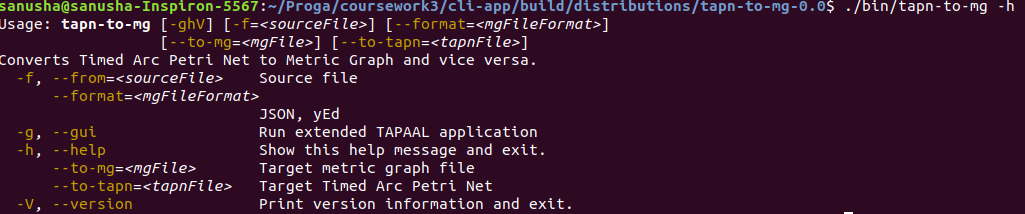
\includegraphics[width=0.7\linewidth]{help}
			\caption{Справка по программе}
			\label{fig:help}
		\end{figure}
		
		\subsection{Запуск конвертации метрического графа в временную сеть Петри}\label{subsection:mg-to-tapn}
		Для запуска конвертации нужно указать ключ -f/--from с исходным файлом, и --to-tapn с путем, до результата
		\begin{figure}[h!]
			\centering
			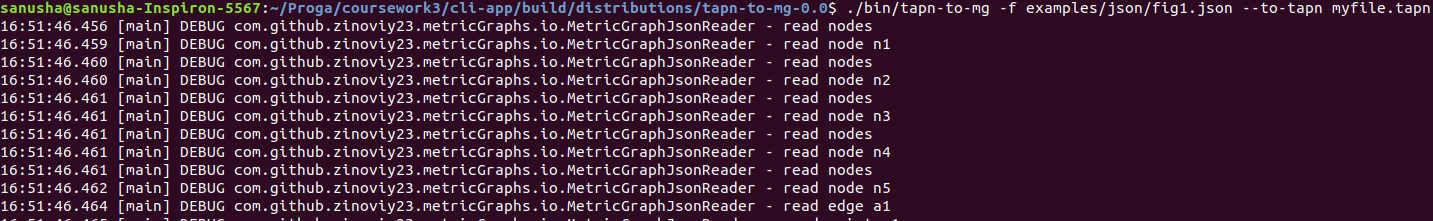
\includegraphics[width=0.7\linewidth]{mg-to-tapn}
			\caption{Конвертация из метрического графа, в сеть Петри}
			\label{fig:mg-to-tapn}
		\end{figure}
		
		\subsection{Запуск конвертации временной сети Петри в метрический граф}\label{subsection:tapn-to-mg}
			Для запуска конвертации нужно указать ключ -f/--from с исходным файлом, и --to-mg с путем, до результата, и опциаональным флагом --format, указав значение json или yed (по умолчанию json) для обозначения выходного формата.
		\begin{figure}[h!]
			\centering
			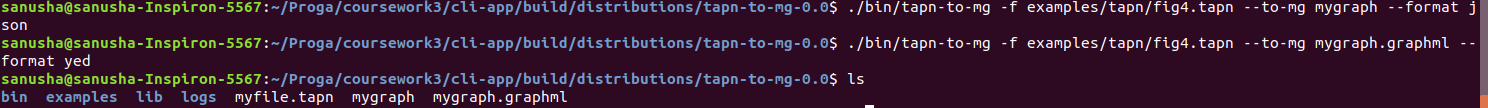
\includegraphics[width=0.7\linewidth]{tapn-to-mg}
			\caption{Конвертация из временной сети Петри в метрический граф}
			\label{fig:tapn-to-mg}
		\end{figure}
		
		\subsection{Запуск расширенного TAPAAL}
		Пункты \ref{subsection:mg-to-tapn}, \ref{subsection:tapn-to-mg} можно так-же произвести в расширенном TAPAAL. Для этого нужно передать ключ -g/--gui, и опиционально -f, для выбора файла
		\begin{figure}[h!]
			\centering
			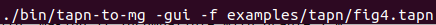
\includegraphics[width=0.7\linewidth]{tapaal-run}
			\caption{запуск расширенного TAPPAL}
			\label{fig:tapaal-run}
		\end{figure}
	
		\begin{figure}[h!]
			\centering
			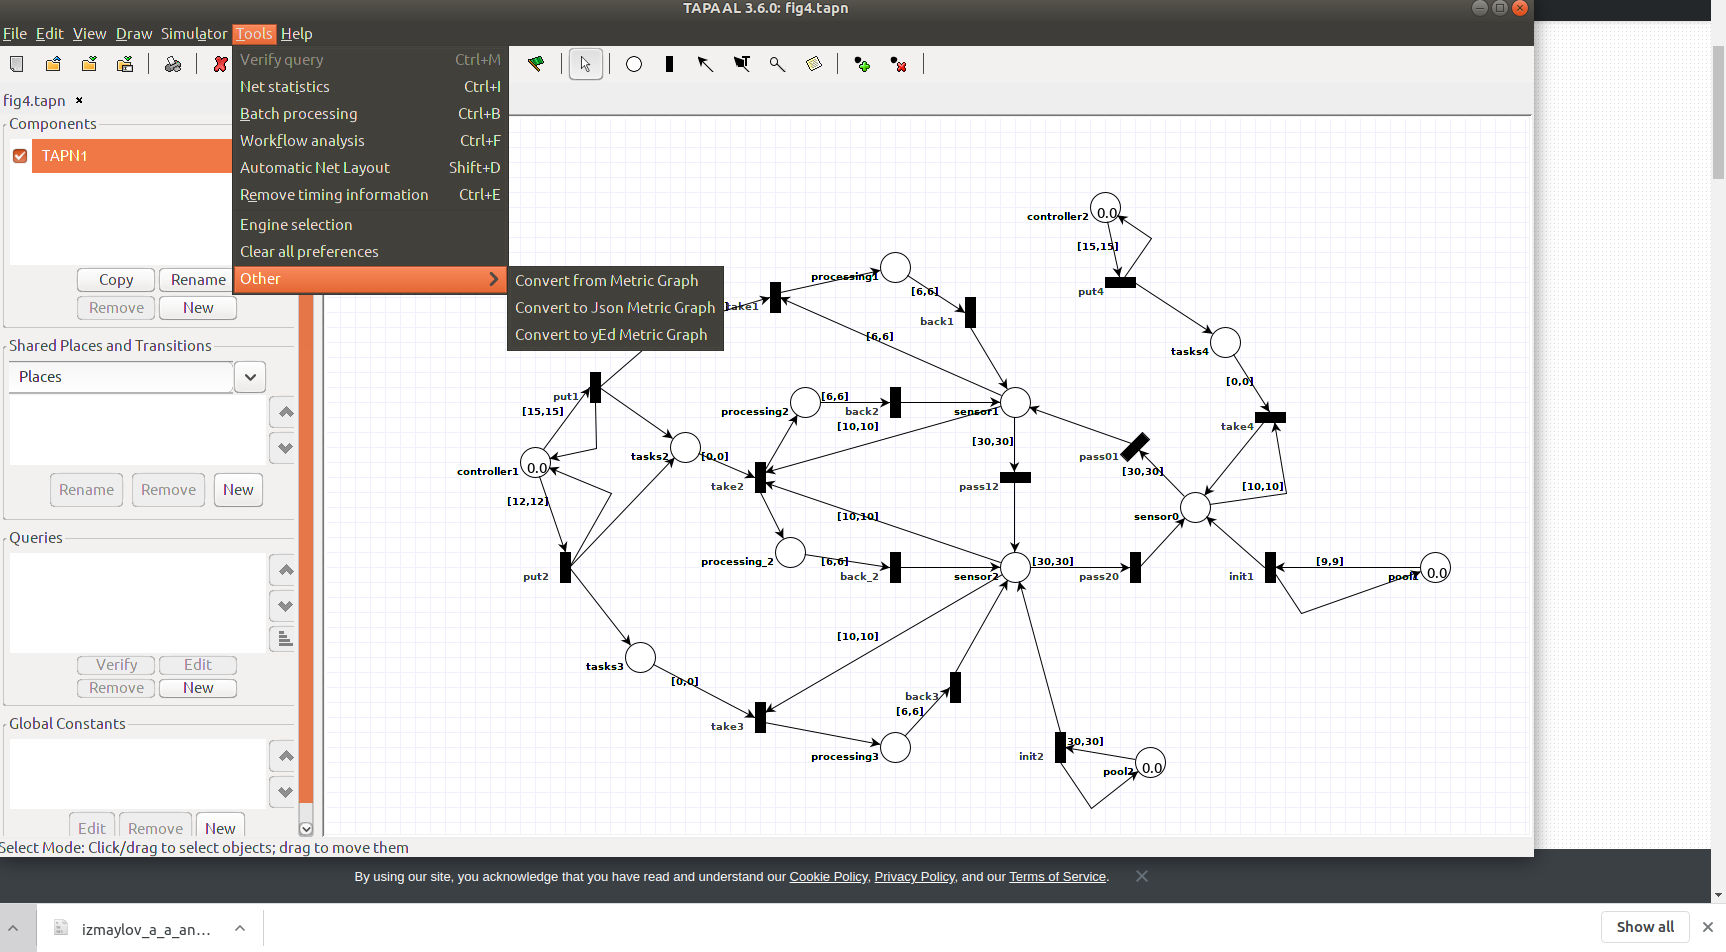
\includegraphics[width=0.9\linewidth]{tapaal-menu}
			\caption{меню для конвертаций, анологичным из пункта \ref{subsection:mg-to-tapn}, \ref{subsection:tapn-to-mg}}
			\label{fig:tapaal-menu}
		\end{figure}
		
	\section{Сообщение пользователю}
		\subsection{Неверный формат временной сети Петри}
		\begin{figure}[h!]
			\centering
			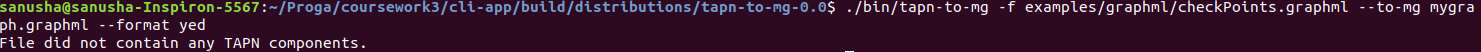
\includegraphics[width=0.7\linewidth]{tapn-format}
			\caption{Ошибка о неправильном формате временной сети петри}
			\label{fig:tapn-format}
		\end{figure}
		\subsection{Сеть Петри не может быть сконвертирована в метрический граф}\label{tapn-error}
		\begin{figure}[h!]
			\centering
			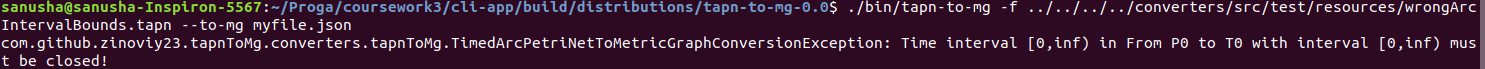
\includegraphics[width=0.7\linewidth]{tapn-format1}
			\caption{Неправильная структура сети Петри}
			\label{fig:tapn-format1}
		\end{figure}
		
		\subsection{Несуществующий файл}
		\begin{figure}[h!]
			\centering
			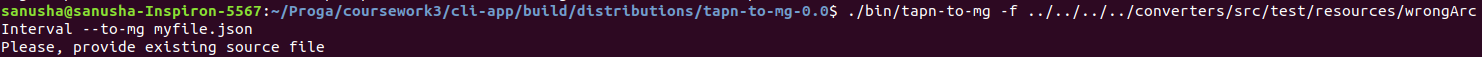
\includegraphics[width=0.7\linewidth]{missing_file}
			\caption{Сообщение о несуществовании входного файла}
			\label{fig:missingfile}
		\end{figure}
	
		\subsection{Уведомление о сохраненом файле}
		\begin{figure}[h!]
			\centering
			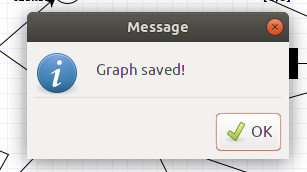
\includegraphics[width=0.7\linewidth]{graph_saved}
			\caption{Уведомление, что сконвертированный граф из текущей сети Петри сохранен}
			\label{fig:graphsaved}
		\end{figure}
		
		\subsection{Сеть Петри не может быть сконвертирована в метрический граф в TAPAAL}
		Внутри TAPAAL также есть все сообщения, о невалидной конвертации, что есть в пункте \ref{tapn-error}
		\begin{figure}[h!]
			\centering
			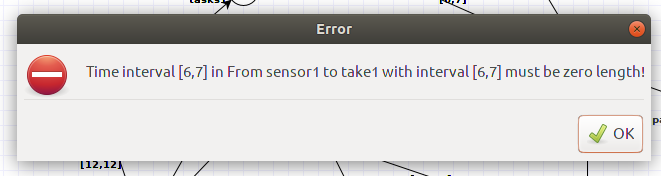
\includegraphics[width=0.7\linewidth]{tapn-format2}
			\caption{Неправильная структура сети Петри}
			\label{fig:tapn-format2}
		\end{figure}
		
		\subsection{Предупреждение о сохранении}
		При конвертации из метрического графа в сеть Петри внутри TAPAAL полученную сеть нужно специально сохранять через "Save as...".
		\begin{figure}[h!]
			\centering
			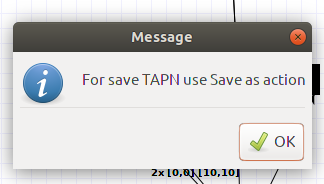
\includegraphics[width=0.7\linewidth]{save}
			\caption{Оповещение о сохранении}
			\label{fig:save}
		\end{figure}
		\registrationList
		
\end{document}